\section{力的图示}\label{sec:2-6}

用手拉弹簧,用的力越大,弹簧伸得越长。这表明力产生的效果跟力的大小有关系,力越大,产生的效果越明显。
用同样大小的力拉弹簧和压弹簧,拉的时候弹簧伸长,压的时候弹簧缩短(图 \ref{fig:2-12})。
这表明力产生的效果还跟力的作用方向有关系。
因此,要表示一个力,只说明它的大小是不够的,还必须同时指出它的方向。
这是力与我们前面学过的长度、质量等物理量不同的地方。
对于长度和质量,我们只要说明它们的大小就行了。

\begin{figure}[htbp]
    \centering
    \begin{minipage}{4cm}
    \centering
    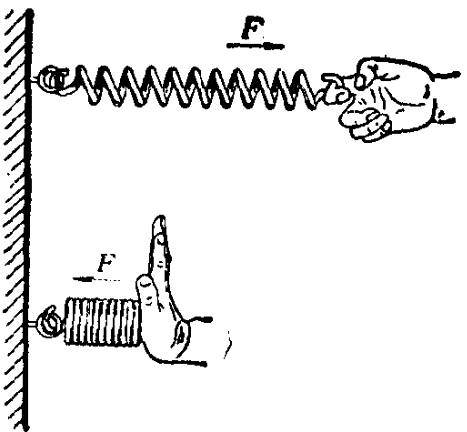
\includegraphics[width=4cm]{../pic/czwl1-ch2-12}
    \caption{}\label{fig:2-12}
    \end{minipage}
    \qquad
    \begin{minipage}{7cm}
    \centering
    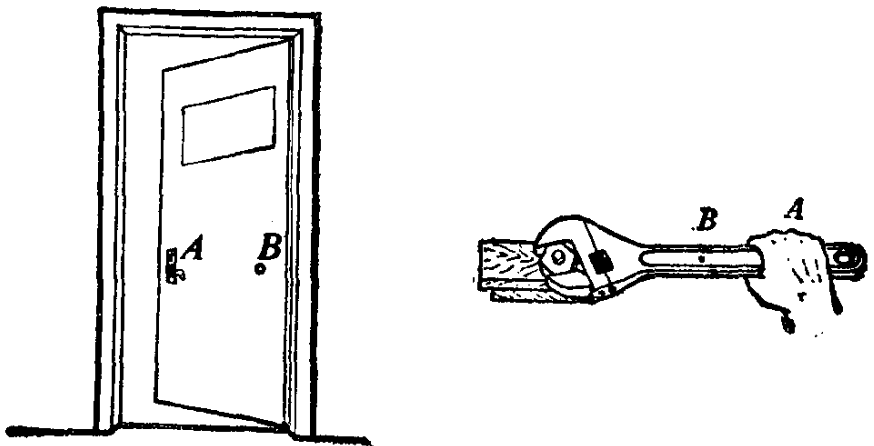
\includegraphics[width=7cm]{../pic/czwl1-ch2-13}
    \caption{}\label{fig:2-13}
    \end{minipage}
\end{figure}

此外,力的作用效果还跟力在物体上的作用点有关系。
例如,开门的时候,推离门轴较远的 $A$ 点比推离门轴较近的 $B$ 点省力。
用扳手拧螺母的时候,手握在把的 $A$ 点比在 $B$ 点省力(图 \ref{fig:2-13})。

\textbf{力的大小、方向和作用点叫做力的三要素}。

我们可以用一根带箭头的线段来表示力,把力的三要素都表示出来。
具体的作法是:从力的作用点起,沿力的方向画一条线段,使线段的长跟力的大小成正比。
例如,用 $3$ 毫米长的线段表示 $10$ 牛顿的力,那么 $30$ 牛顿的力就用 $9$ 亳米长的线段来表示。
最后再在线段的末端画上箭头,表示力的方向(图 \ref{fig:2-14} 甲)。
这种表示力的方法叫做\CJKunderwave{力的图示}。

\begin{figure}[htbp]
    \centering
    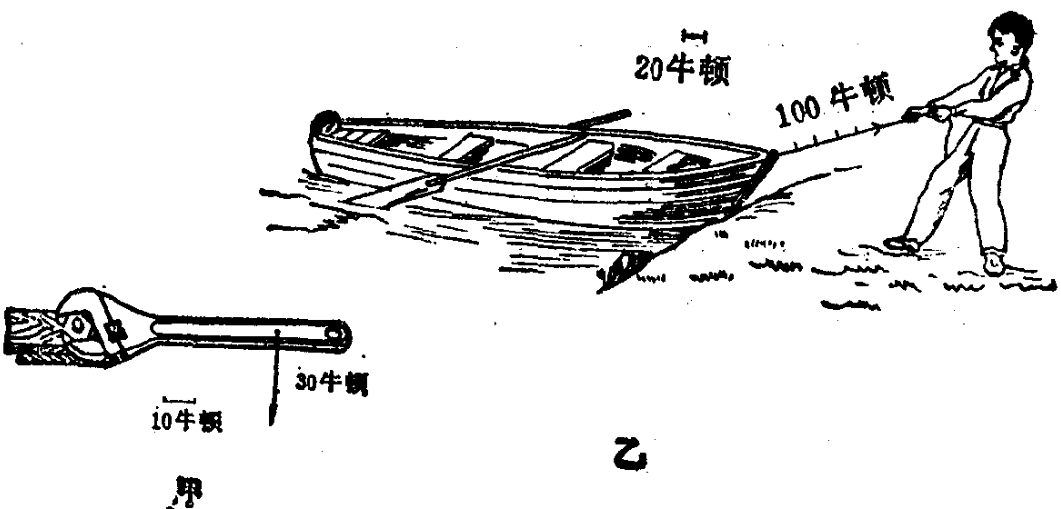
\includegraphics[width=0.6\textwidth]{../pic/czwl1-ch2-14}
    \caption{}\label{fig:2-14}
\end{figure}

用绳子拉小船的时候,作用在小船上的力的方向是沿着绳子的,如果所用的拉力是 $100$ 牛顿,那么小船受到的力如图 \ref{fig:2-14} 乙所示。
因为力总是作用在物体上的,所以作力的图示时,力的作用点一定要画在受力物体上。

物体受到的重力的方向是竖直向下的。重力在物体上的作用点,叫做物体的重心。
均匀直棒的重心在棒的中点,均匀圆盘的重心在盘的中心,均匀圆球的重心在球心,均匀方板的重心在两条对角线的交点。
图 \ref{fig:2-15} 表示一块方板和一个圆球受到的重力。

\begin{figure}[htbp]
    \centering
    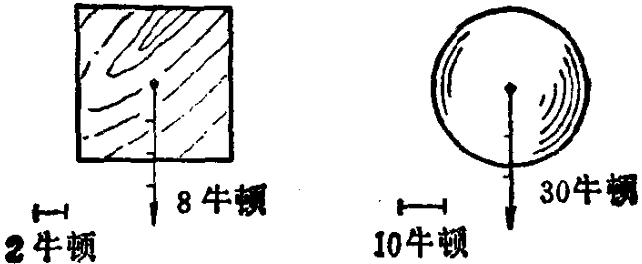
\includegraphics[width=0.6\textwidth]{../pic/czwl1-ch2-15}
    \caption{}\label{fig:2-15}
\end{figure}

在很多情况下不需要严格地按照力的图示法去画力,而只沿力的方向画个箭头表示物体受到力的作用,不严格追究箭头的起点和长度。
这种画法叫做力的示意图,在以后的学习中会经常遇到。


\lianxi

用力的图示法画出下面的力:

(1) 用 200 牛顿的力提面袋;

(2) 用 50 牛顿的力沿水平方向推桌子;

(3) 质量为 30 千克的木箱受到的重力;

(4) 用与地面成 $30^\circ$ 角的力拉小车,拉力为 100 牛顿。


